\documentclass[12pt]{article}
\usepackage[left=2.5cm, right=2.5cm, top=3cm, bottom=3cm]{geometry}
\linespread{1.1}
\frenchspacing

\usepackage{setspace}
%\usepackage{footnote}
%\makesavenoteenv{tabular}
%\makesavenoteenv{table}
\usepackage{tablefootnote}
\usepackage{natbib}
\usepackage[utf8]{inputenc}
\usepackage[english]{babel}
\usepackage{amsmath}
\usepackage{amsfonts}
\usepackage{amssymb}
\usepackage{mathtools}
\usepackage{stmaryrd}
\usepackage{amsthm}
\usepackage{thmtools}
\usepackage{tikz}
\usetikzlibrary{calc}
\usepackage{graphicx}
\usepackage{mathrsfs}
\usepackage{mathdots}
\usepackage{listings}
\usepackage[linesnumbered, ruled, vlined]{algorithm2e}
\usepackage[inline]{enumitem}
\usepackage{wrapfig}
\usepackage{float}
\usepackage{array}
\usepackage[justification=centering]{caption}
\usepackage{subcaption}
\usepackage{epigraph}
\usepackage{xspace}
\usetikzlibrary{arrows, automata, graphs, shapes, petri, decorations.pathmorphing}
\usepackage{hyperref}
\usepackage{unicode-math}
\unimathsetup{math-style=ISO, partial=upright, nabla=upright}
\defaultfontfeatures{Scale=MatchLowercase}
\setmainfont[Numbers={OldStyle,Proportional}]{TeX Gyre Pagella}
\usepackage[OT1, euler-digits, euler-hat-accent]{eulervm}
\setmathfont{euler}
\setmathfont[range={up/num, bfup/num, it, bfit, scr, bfscr,
                    sfup, sfit, bfsfup, bfsfit, tt} 
            ]{Asana Math}
\setmathfont[range=bfcal, Scale=MatchUppercase, Alternate]{Asana Math}
\setmathfont[range=bb, Scale=MatchUppercase]{Asana Math}

\newcommand{\cmd}[1]{\colorbox{red!20}{\textcolor{red!90}{\texttt{#1}}}}
\newcommand{\code}[1]{\texttt{#1}}
\usepackage{pgfplots}
\pgfplotsset{compat=1.13}
\pgfmathdeclarefunction{gauss}{2}{%
  \pgfmathparse{1/(#2*sqrt(2*pi))*exp(-((x-#1)^2)/(2*#2^2))}%
}

\lstset{showstringspaces=false, columns=flexible, framesep=10pt, language=bash, breaklines=true, breakatwhitespace=false, backgroundcolor=\color{black}, basicstyle=\small\ttfamily\color{white}, rulecolor=\color{gray}}

\title{Der Satz von Taylor}
\author{Niklas Rieken}


\begin{document}
\maketitle

Wir können beliebige stetig differenzierbarbare Funktionen $f\colon A \to \mathbb{R}$ mit $A \subseteq \mathbb{R}$ in der Umgebung eines Punktes (der \emph{Entwicklungsstelle}) $a \in A$ durch \emph{Taylorpolynome} $T_nf(x; a)$. Diese haben die Eigenschaft, dass sie bis zur $n$-ten Ableitung in der Entwicklungsstelle mit der ursprünglichen Funktion $f$ übereinstimmt und damit auch in einer Umgebung von $a$, nicht zu weit abweicht von $f$. Da $T_nf$ ein Polynom ist lässt sich damit oft deutlich einfacher arbeiten als mit $f$.

Das \emph{$n$-te Taylorpolynom} im Entwicklungspunkt $a$ ist definiert als:
\begin{align*}
	T_nf(x; a) &= \sum_{k=0}^n \frac{f^{(k)}(a)}{k!} (x-a)^k\\
	&= f(a) + f'(a) (x-a) + \tfrac{1}{2} f''(a) (x-a)^2 + \tfrac{1}{6} f'''(a) (x-a)^3 + \ldots + \tfrac{1}{n!} f^{(n)}(a) (x-a)^n.
\end{align*}

D.h. das $0$-te Taylorpolynom ist einfach eine Konstante mit dem Funktionswert von $f$ in $a$. Das Taylorpolynom von Grad $1$ besitzt zusätzlich die erste Ableitung gleich der zu approximierenden Funktion in der Stützstelle, damit sind auch benachbarte Punkte relativ exakt approximiert (man erinnert sich, dass die Idee einer Ableitung bzw. von Differenzierbarkeit ist, dass Funktionen auf sehr kleinen Intervallen eben fast linear verlaufen). Das $2$-te Taylorpolynom hat entsprechend auch noch die zweite Ableitung in $a$ gleich der zweiten Ableitung der Funktion usw. Intuitiv gesehen schmiegen sich die Taylorpolynome immer mehr der ursprünglichen Funktion an.

\begin{figure}
	\centering
	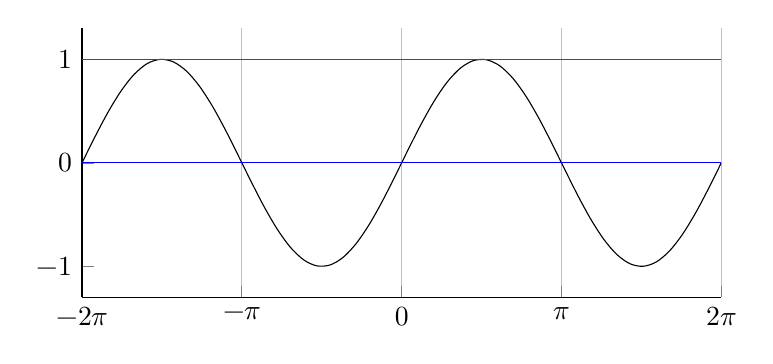
\begin{tikzpicture}
		\begin{axis}[
			width=.8\textwidth, height=5cm,
			domain=-2*pi:2*pi,samples=50,smooth,
			ymin=-1, ymax=1,
			axis x line*=bottom, % no box around the plot, only x and y axis
			axis y line*=left, % the * suppresses the arrow tips
			xtick = {-6.283, -3.145, 0, 3.1415, 6.283},
			xticklabels = {$-2\pi$, $-\pi$, 0, $\pi$, $2\pi$},
			grid = major, ymajorgrids = false,
			x tick label style={black},
			enlarge y limits=.15, enlarge x limits=0]
			\addplot[mark=none]{sin(deg(x))};
			\addplot[mark=none, color=blue]{0};
			\addplot[mark=none, color=red]{1};
		\end{axis}
	\end{tikzpicture}
	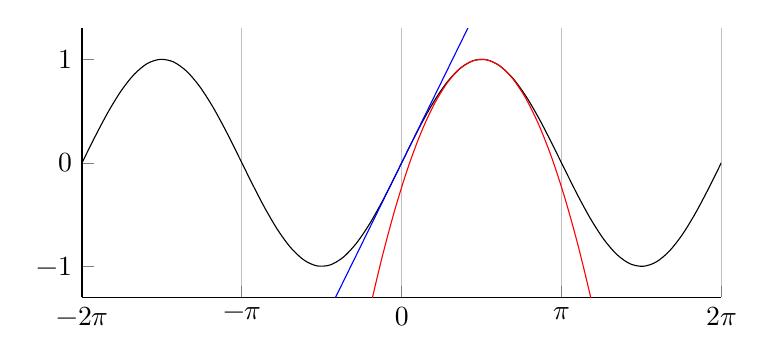
\begin{tikzpicture}
		\begin{axis}[
			width=.8\textwidth, height=5cm,
			domain=-2*pi:2*pi,samples=50,smooth,
			ymin=-1, ymax=1,
			axis x line*=bottom, % no box around the plot, only x and y axis
			axis y line*=left, % the * suppresses the arrow tips
			xtick = {-6.283, -3.145, 0, 3.1415, 6.283},
			xticklabels = {$-2\pi$, $-\pi$, 0, $\pi$, $2\pi$},
			grid = major, ymajorgrids = false,
			x tick label style={black},
			enlarge y limits=.15, enlarge x limits=0]
			\addplot[mark=none]{sin(deg(x))};
			\addplot[mark=none, color=blue]{x};
			\addplot[mark=none, color=red]{1 - ((x-pi/2)^2)/2};
		\end{axis}
	\end{tikzpicture}
	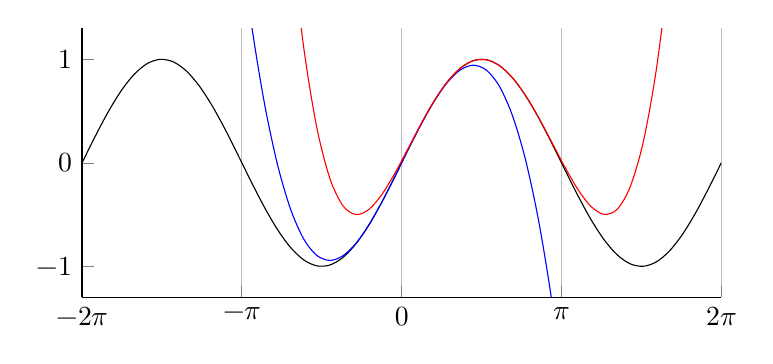
\begin{tikzpicture}
		\begin{axis}[
			width=.8\textwidth, height=5cm,
			domain=-2*pi:2*pi,samples=50,smooth,
			ymin=-1, ymax=1,
			axis x line*=bottom, % no box around the plot, only x and y axis
			axis y line*=left, % the * suppresses the arrow tips
			xtick = {-6.283, -3.145, 0, 3.1415, 6.283},
			xticklabels = {$-2\pi$, $-\pi$, 0, $\pi$, $2\pi$},
			grid = major, ymajorgrids = false,
			x tick label style={black},
			enlarge y limits=.15, enlarge x limits=0]
			\addplot[mark=none]{sin(deg(x))};
			\addplot[mark=none, color=blue]{-1/6*x^3 + x};
			\addplot[mark=none, color=red]{1 - ((x-pi/2)^2)/2 + ((x-pi/2)^4)/24};
		\end{axis}
	\end{tikzpicture}
	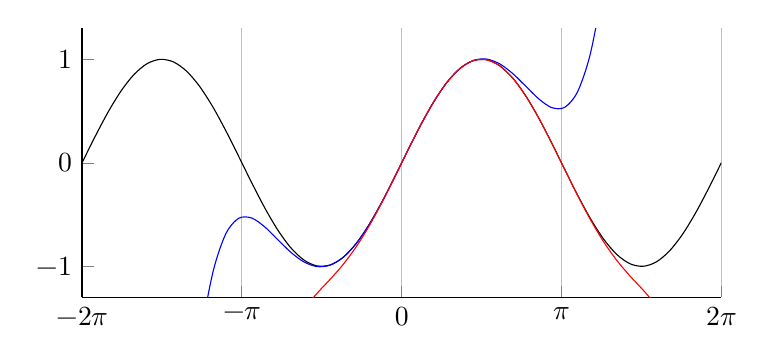
\begin{tikzpicture}
		\begin{axis}[
			width=.8\textwidth, height=5cm,
			domain=-2*pi:2*pi,samples=50,smooth,
			ymin=-1, ymax=1,
			axis x line*=bottom, % no box around the plot, only x and y axis
			axis y line*=left, % the * suppresses the arrow tips
			xtick = {-6.283, -3.145, 0, 3.1415, 6.283},
			xticklabels = {$-2\pi$, $-\pi$, 0, $\pi$, $2\pi$},
			grid = major, ymajorgrids = false,
			x tick label style={black},
			enlarge y limits=.15, enlarge x limits=0]
			\addplot[mark=none]{sin(deg(x))};
			\addplot[mark=none, color=blue]{1/120*x^5 - 1/6*x^3 + x};
			\addplot[mark=none, color=red]{1 - ((x-pi/2)^2)/2 + ((x-pi/2)^4)/24 - ((x-pi/2)^6)/720};
		\end{axis}
	\end{tikzpicture}
	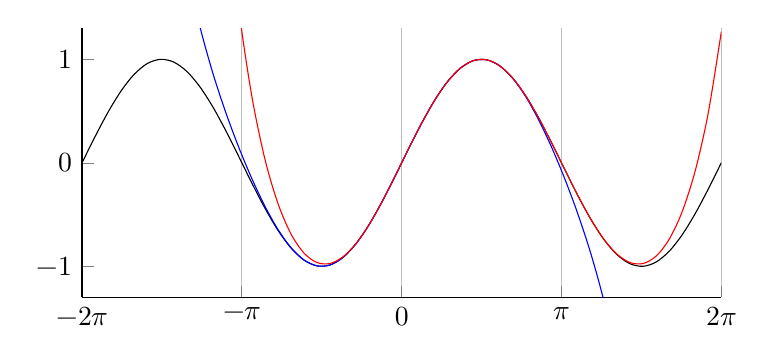
\begin{tikzpicture}
		\begin{axis}[
			width=.8\textwidth, height=5cm,
			domain=-2*pi:2*pi,samples=50,smooth,
			ymin=-1, ymax=1,
			axis x line*=bottom, % no box around the plot, only x and y axis
			axis y line*=left, % the * suppresses the arrow tips
			xtick = {-6.283, -3.145, 0, 3.1415, 6.283},
			xticklabels = {$-2\pi$, $-\pi$, 0, $\pi$, $2\pi$},
			grid = major, ymajorgrids = false,
			x tick label style={black},
			enlarge y limits=.15, enlarge x limits=0]
			\addplot[mark=none]{sin(deg(x))};
			\addplot[mark=none, color=blue]{-1/5040*x^7 + 1/120*x^5 - 1/6*x^3 + x};
			\addplot[mark=none, color=red]{1 - ((x-pi/2)^2)/2 + ((x-pi/2)^4)/24 - ((x-pi/2)^6)/720 + ((x-pi/2)^8)/40320};
		\end{axis}
	\end{tikzpicture}
	\caption{Sinus-Funktion und Taylorpolynome von Grad $0$, $1$, $3$, $5$, $7$ mit Entwicklungspunkt $0$ (blau) und von Grad $0$, $2$, $4$, $6$, $8$ mit Entwicklungspunkt $\tfrac{\pi}{2}$ (rot). Beachte, dass für $T_{2n}\sin(x; 0) = T_{2n-1}\sin(x; 0)$ für $n \geq 1$ und $T_{2n}\sin(x; \frac{\pi}{2}) = T_{2n+1}\sin(x; \frac{\pi}{2})$ für $n \geq 0$.}
	\label{fig:taylorsinus}
\end{figure}

\end{document}
